% Version 2022-09-20
% update – 161114 by Ken Arroyo Ohori: made spacing closer to Word template throughout, put proper quotes everywhere, removed spacing that could cause labels to be wrong, added non-breaking and inter-sentence spacing where applicable, removed explicit newlines
% update – 010819 by Dennis Wittich: made spacing and font size closer to Word template, updated references and refernces style
% update – 042319 by Dennis Wittich: font size of captions set to 'small', first author names are shortened, hyphenation fixed
% update – 010620 by Dennis Wittich: Footnotes alignment set to left
% update - 151220 by Clement Mallet: Template adapted for double blind full paper submissions
% update - 060321 by Christian Heipke: Template refined for double blind full paper submissions
% update - 090921 by Christian Heipke: Template refined for double blind full paper submissions
% update - 200922 by Christian Heipke: general template update
% update - 080124 by Christian Heipke: general template update

\documentclass{isprs} % isprs class modified 23-04-2019 (Dennis Wittich)
\usepackage{subfigure}
\usepackage{setspace}
\usepackage{geometry} % added 27-02-2014 Markus Englich
\usepackage{epstopdf}
\usepackage[labelsep=period]{caption}  % added 14-04-2016 Markus Englich - Recommendation by Sebastian Brocks
\usepackage[british]{babel} 
\usepackage[hang]{footmisc}
\usepackage{graphicx} % Pacote necessário para imagens
\usepackage{url}  % URL handle
\def\footnotemargin{1em} % added 08-01-2020 Dennis Wittich

%\usepackage[authoryear]{natbib}
%\def\bibhang{0pt}

\geometry{a4paper, top=25mm, left=20mm, right=20mm, bottom=25mm, headsep=10mm, footskip=12mm} % added 27-02-2014 Markus Englich
%\usepackage{enumitem}

%\usepackage{isprs}
%\usepackage[perpage,para,symbol*]{footmisc}

%\renewcommand*{\thefootnote}{\fnsymbol{footnote}}
\captionsetup{justification=centering,font=normal} % thanks to Niclas Borlin 05-05-2016
\captionsetup[figure]{font=small} % added 23-04-2019 Dennis Wittich
\captionsetup[table]{font=small} % added 23-04-2019 Dennis Wittich

\begin{document}

\title{A case use of FOSS4G to promote the Mining Industry: The P3M Platform of the Geological Survey of Brazil}
\date{}


% KAO: Remove extra spacing

% Anonymous submissions, authors' names should not be visible
\author{
	Carlos Eduardo Miranda Mota\textsuperscript{1}, 
	Gilberto Dias Calaes\textsuperscript{2}, 
	Luís Fernando Barbosa de Almeida\textsuperscript{3}, 
	Paulo Cesar Barbosa Junior\textsuperscript{3}, 
	José Luciano Stropper\textsuperscript{3},
	Amaro Luiz Ferreira\textsuperscript{1},
	Ricardo Terra\textsuperscript{4},
	Junior Cezar Avanzi\textsuperscript{5},
	André Pimenta Freire\textsuperscript{4}
}

% KAO: Remove extra newline
% Anonymous submissions, authors' affiliations should not be visible
\address{
	\textsuperscript{1 }Department of Institutional Information, Geological Survey of Brazil - (carlos.mota, amaro.ferreira)@sgb.gov.br\\
	\textsuperscript{2 }CONDET Business Consulting Ltd, Brazil\\
	\textsuperscript{3 }Department of Mineral Resources, Geological Survey of Brazil\\
	\textsuperscript{4 }Department of Computer Science, Federal University of Lavras, Brazil\\
	\textsuperscript{5 }Department of Soil Science, Federal University of Lavras, Brazil\\
}

% If the corresponding author is NOT the final author, always add a % space before the subsequent comma, i.e.
% first author name\textsuperscript{a,}\thanks{Corresponding author} , % second author name \textsuperscript{b}, etc.
% thanks to Niclas Borlin 05-05-2016
% information on the corresponding author should not be used any longer and has been commented out
% C. Heipke, Jan 03,2024

% the use of the information of commissions and working groups should not be used any longer and has been commented out
% C. Heipke, Sept. 20,2022
%\commission{XX, }{YY} %This field is optional. If filled, XX and YY should be replaced by adequate numbers. See https://www2.isprs.org/commissions/
%\workinggroup{XX/YY} %This field is optional.
%\icwg{}   %This field is optional.


% KAO: Use times symbol
\abstract{
The P3M Platform, developed by the Brazilian Geological Survey (SGB), is a strategic tool for planning national mineral research and production. Its central differentiator is its design based entirely on free software (FOSS4G), which ensures transparency, interoperability, and independence from restrictive proprietary licensing. The architecture uses open-source technologies such as PostgreSQL/PostGIS for storage, Django and OpenLayers for interfaces, and Apache Airflow for orchestrating data flows. Strictly following OGC standards, the platform integrates approximately 320 layers of geoscientific, environmental, and socioeconomic information into a one-stop-shopping hub. This robust infrastructure enhances strategic decision-making and promotes the sustainability and competitiveness of the sector, consolidating P3M as an essential database for attracting investment and sustainable development.
}

\keywords{Mineral Exploration, Mineral Research, Mineral Resources, Dashboard, Web Mapping, FOSS4G}

\maketitle


% KAO: Sloppy spacing ensures non-overfull lines. Can be removed if this is not an issue.
\sloppy


\section{Introduction}\label{INTRDUCTION}

The Mineral Research and Production Support Platform (P3M) was conceived and is being implemented by a team of specialists from the Geological Survey of Brazil (SGB), with the support and participation of public and private entities directly or indirectly related to the Brazilian mineral industry, such as: Secretariat of Geology, Mining and Mineral Transformation (SGM) of the Ministry of Mines and Energy (MME); National Mining Agency (ANM); Agency for the Development and Innovation of the Brazilian Mineral Sector (ADIMB); Brazilian Association of Mineral Research and Mining Companies (ABPM); National Association of Aggregate Producers for Construction (ANEPAC); Brazilian Institute of Geography and Statistics (IBGE), and Brazilian Mining Institute (IBRAM).

The core development of P3M is being carried out by the UFLA (Federal University of Lavras) Agency for Innovation in Geotechnologies and Intelligent Systems (Zetta). Launched in late 2022, the P3M's main objective is to increase the attractiveness of investments and promote the sustainable development of the mineral industry, through the integration of data on mineral potential, infrastructure, costs, legislation, protected areas, and socioeconomic indicators of Brazil. The P3M's landing page (Figure~\ref{fig:p3m_architecture}) is hosted on \url{https://p3m.sgb.gov.br/} and has auto-translated versions in english and spanish.

\begin{figure}[ht!]
    \begin{center}
        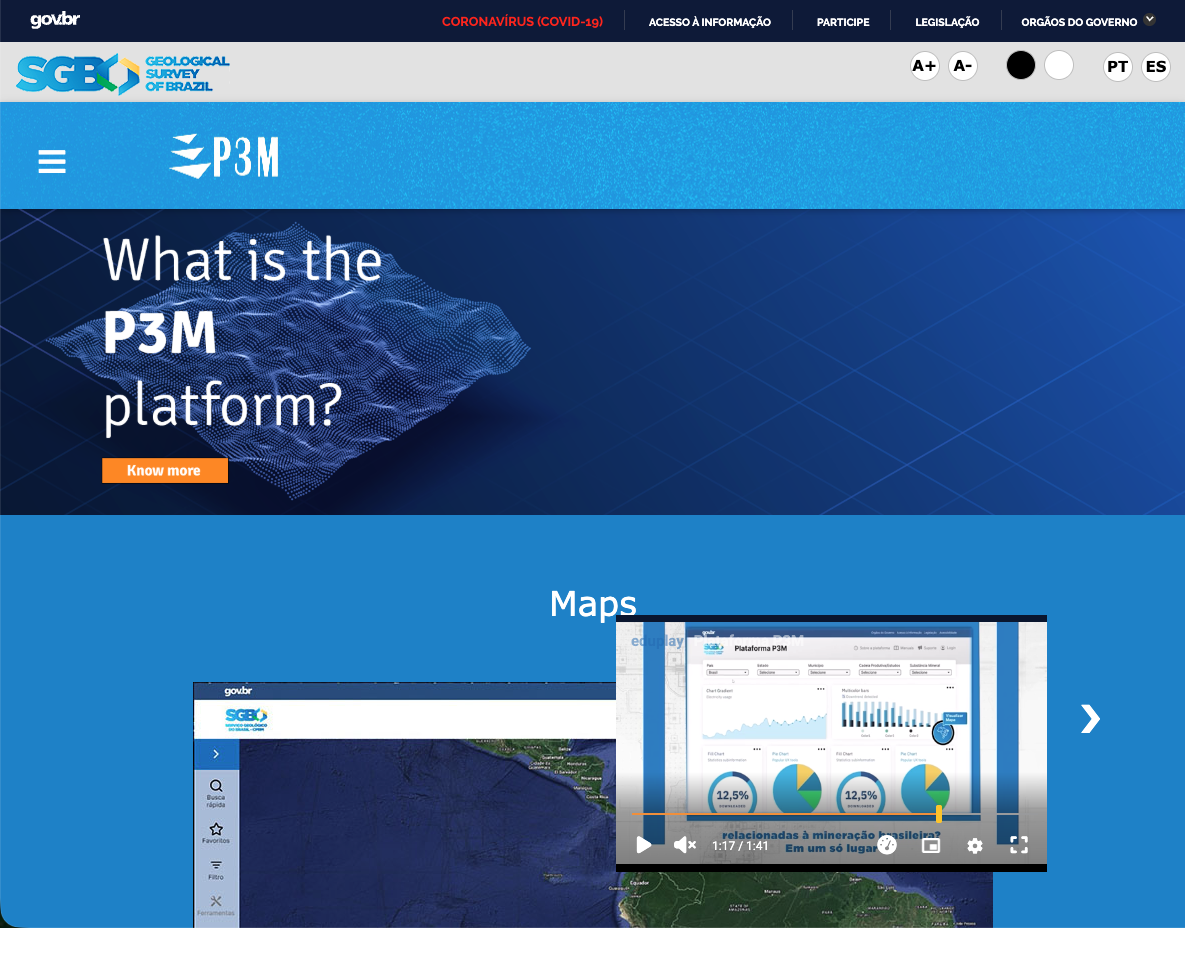
\includegraphics[width=1.0\columnwidth]{images/p3m_website.png}
        \caption{Landing page of P3M platform, with information and access for the web application}
        \label{fig:p3m_website}
    \end{center}
\end{figure}

It has a crucial role in planning mineral research and production, generating qualified knowledge that is essential to support strategic decisions in both the public and private sectors. For industries and investors in the mining sector, the data available on the Platform contribute to supporting development plans and the exploitation of mineral deposits. Government entities also benefit primarily from information for monitoring the competitiveness of mineral research and production, thereby promoting greater attractiveness of investments for national development.

In short, P3M provides information free of charge through two main environments: (i) a map and data viewer that integrates geoscientific, economic, environmental and legal information, mining rights, among others, from various national and governmental entities; and (ii) a dashboard system with statistical data presentation, with filters by territorial unit (e.g., region, state, or municipality) and commodity \cite{almeida2025}.

One of the main differentiators of the P3M platform, among the various software products of SGB, is its complete conception and development using FOSS4G. The main objective of this work is to present the solution architecture used in the development, focusing primarily on the use of FOSS4G projects. In early February of this year, version 2.4.4 was released, with several improvements in terms of user experience and performance.


\section{System Architecture}\label{SYSTEM_ARCHITECTURE}

In general terms, the P3M Platform can be subdivided into three main components: (i) Web Map and Dashboard visualization system: This provides a responsible user interface with web maps and integrated dashboards filtered by commodity (copper, lead, gold or silver for example) or class of commodities (metallic minerals), and Economy Mineral dashboards in a BI system that can be filtered dynamically by Brazilian territory subdivisions or mineral substance, (ii) Data Pipeline orchestration: this component has the role to feed the P3M databases with updated information of mining processes and ventures from Brazilian Mining Agency into a set of scheduled pipelines, and (iii) spatial data infrastructure, that provides map layers, data and metadata for the web map application (Figure~\ref{fig:p3m_architecture}). 

\begin{figure}[ht!]
    \begin{center}
        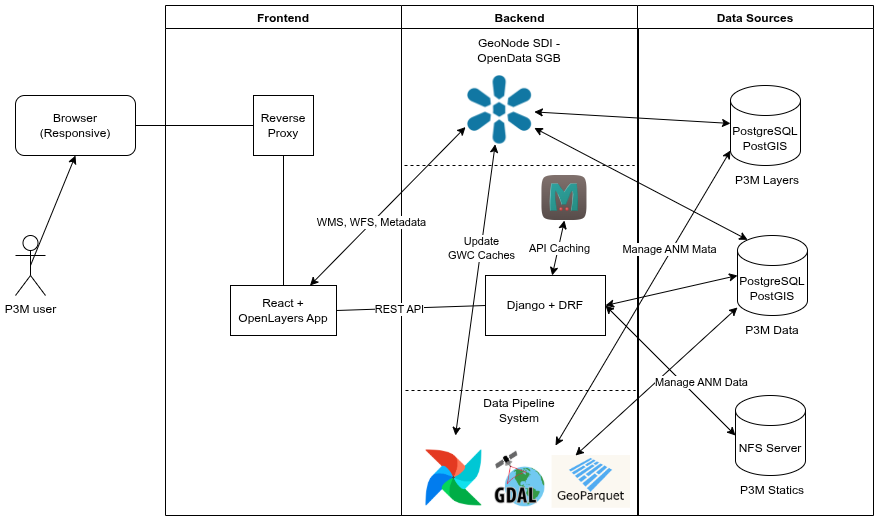
\includegraphics[width=1.0\columnwidth]{images/arquitetura_p3m.drawio.png}
        \caption{System architecture of P3M, integrated to SGB's SDI as map sources}
        \label{fig:p3m_architecture}
    \end{center}
\end{figure}

The platform's deployment is entirely cloud-ready, provisioned on a on-premise OpenShift Cluster \cite{redhatopenshift} with all implemented security restrictions inside the platform. In other words, all P3M pods run with a random UUID and limited capacities, which improves security. The Kubernetes resources are provisioned with use of Helm Charts \cite{helm2016}. An active CI/CD pipeline is under development at this moment.

The data storage relies on PostgreSQL 14 databases with PostGIS 3.4 \cite{postgis} and NFS servers for raster layers storage. In last quarter of 2026, a database upgrade is scheduled to superseed PostgreSQL version to 17. PostGIS will remain in the same version, because of requirements of parallel projects running inside te DBMS server.


\subsection{Web Map and Dashboards}\label{sec:WEB_MAP_AND_DASHBOARDS}

The map and dashboard applications are deployed into two container images: the first, a backend project with Django \cite{django} + Rest framework \cite{drf}, brings a system of REST APIs to define the content controls for the maps and dashboards and provides structured data to feed the cards and charts. 

To accelerate the delivery of structured data to the REST API, a Memcached deployment was provisioned to store indicator's cached results. This service is implemented natively within the Django framework \cite{django_memcached} and is optional, though recommended for improving API performance.

All these services uses Kubernetes Deployment objects due to their stateless nature (Figure~\ref{fig:p3m_frontend_k8s}). Additionally, a HorizontalPodAutoscaler can optionally be provided via a Helm chart — alongside the Deployment, Service, and Ingress objects—for each frontend and backend pods to ensure horizontal scalability for the services.

\begin{figure}[ht!]
    \begin{center}
        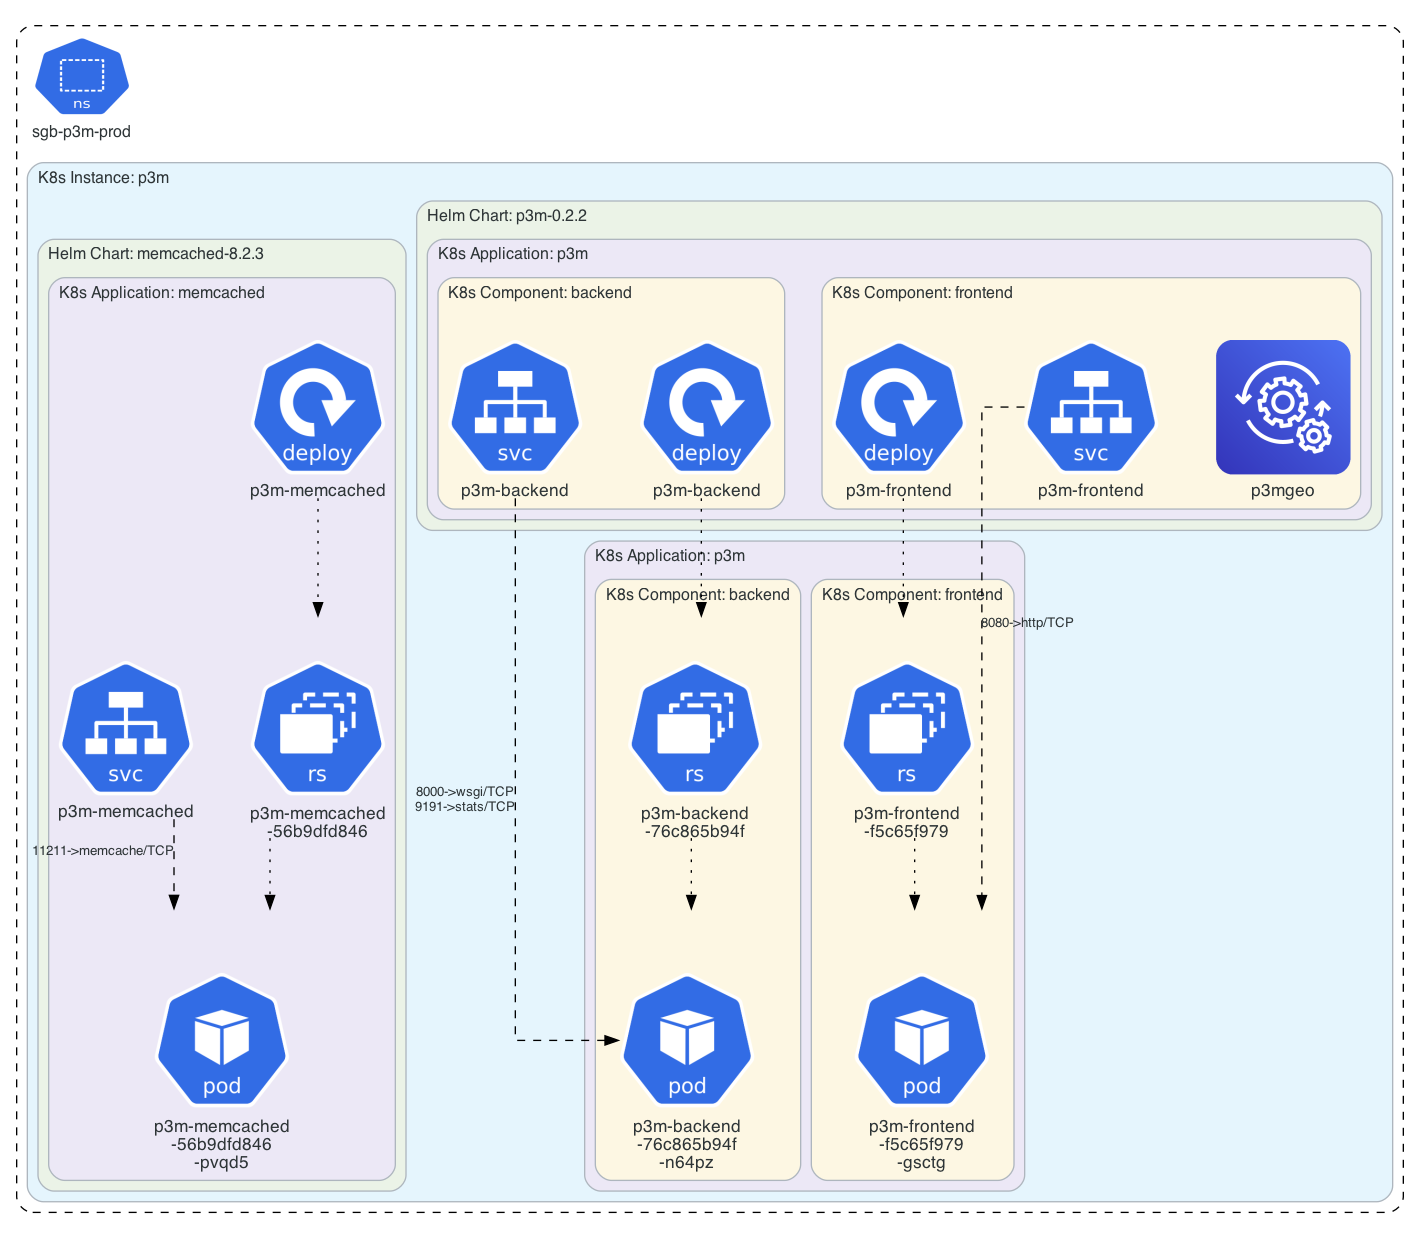
\includegraphics[width=1.0\columnwidth]{images/p3m-k8s-prod.png}
        \caption{Kubernetes implementation of the P3M's Web Map and Dashboard visualization system, generated by KubeDiagrams PyPI package \protect\cite{merle2025}}
        \label{fig:p3m_frontend_k8s}
    \end{center}
\end{figure}

This system does not require persistent disk provisioning for data storage; data files—typically geophysical grids in GeoTIFF format—are hosted on the SGB's GeoNode. Only a ephemeral storage, provided by a NFS server is used to provide static files generated by Django and expose as a read-only mount to the frontend pod.

Furthermore, the application has an administrative interface based on the Django Admin framework,that allows for modifying various application behaviors, as well as registering, editing, and deleting WMS and WFS-compatible layers; describing column attributes and metadata info and links. It also can manage definitions regarding mineral resources, mining clusters, and layer groups organized by mineral substance or commodity.

The front-end component is a TypeScript application that relies on libraries such as OpenLayers \cite{openlayers} and Chart.JS \cite{chartjs} to render the layer tree, delivered by the backend, and the dashboard data into cards and charts. This application were transpiled to Javascript and hosted in nginx web server. \cite{reese2008linux}.


\subsection{Data Pipeline System}\label{sec:DATA_PIPELINE_SYSTEM}

The data pipeline orchestration environment was deployed from a custom Apache Airflow \cite{apacheairflow} container image, supplemented with libraries such as GDAL \cite{gdal} and Apache Arrow/GeoParquet \cite{geoparquet}.

(Figure~\ref{fig:p3m_airflow_schema})

\begin{figure}[ht!]
    \begin{center}
        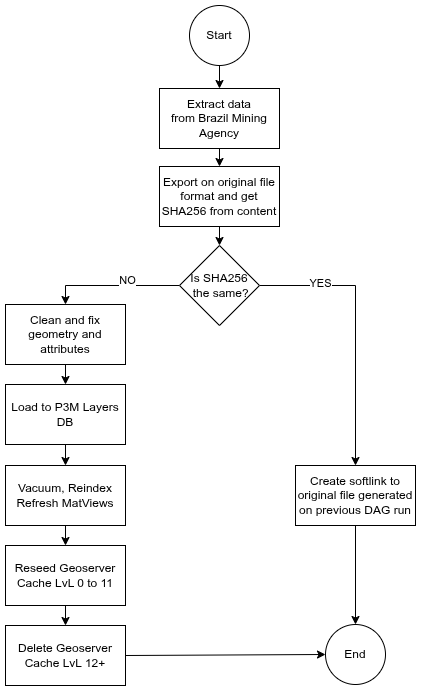
\includegraphics[width=1.0\columnwidth]{images/Airflow_DAG_flux.drawio.png}
        \caption{Simplified outline of the tasks required for Brazilian mining data ETL process, implemented as Apache Airflow DAGs}
        \label{fig:p3m_airflow_schema}
    \end{center}
\end{figure}

For P3M, some data pipelines were developed to collect data of mining processes and financial compensation – available from the National Mining Agency (ANM). This data, originally delivered in spreadsheets and File Geodatabases, is sanitized, enriched, and transformed using GDAL, and finally saved in proprietary PostgreSQL/PostGIS tables of active mines, commodity associations, and mining process statuses. Currently, these pipelines run on Mondays, Wednesdays, and Fridays and are crucial for maintaining the dashboards and authorial layers.


\subsection{Underlying Spatial Data Infrastructure}\label{sec:UNDERLYING_SPATIAL_DATA_INFRASTRUCTURE}

The provision of maps and metadata on P3M strictly follows the use of OGC Open Web Services standards, such as WMS, WMTS, and WFS, and the platform consumes maps and metadata from a GeoNode \cite{geonode_contributors} installation owned by the SGB \cite{mota2024}, in order to fulfill the role of Spatial Data Infrastructure.

The SGB’s GeoNode was deployed to a production environment in late 2025, initially to support this platform. Before this GeoNode, P3M had a dedicated GeoServer instance in its own workspace to serve the maps. After going into production, all layers and configurations were moved to this GeoNode. Currently, about 320 vector and raster layers are cataloged and registered from various Brazilian government data sources. Initially, this data was organized and cleaned to create a database that was placed as a datastore in GeoNode's GeoServer.

The option of hosting duplicate data instead of consuming OGC services from other institutions was chosen due to the need to have these data available on the platform, even if the source provider is unavailable, in addition to the geological service having a robust IT infrastructure. The P3M authorial layers are also hosted on GeoNode, but directly from the exposure of the spatial tables to the GeoNode/Geoserver. Some of these tables, such as mineral resource data and systematic mapping, are also fed from airflow pipelines.


\section{Case Study – Copper Research on Southern Brazil}\label{CASE_STUDY_COPPER_SOUTHERN_BRAZIL}

A typical case use of P3M applied to mineral resource prospecting, cited as an example, was first published by \cite{barbosajunior2025}. This example will simulate an information gathering activity on copper in the state of Rio Grande do Sul, to evaluate potential areas for new research applications for this mineral substance.

The approach involves on platform navigation, starting from the side panel, on "Main Class of Commodities", select metallic minerals $>$ Copper (Cu). From this selection, specific geospatial layers are activated, such as active mines, current mining rights, geological, geochemical and geophysical surveys, as well as occurrences and deposits mapped by the Geological Survey of Brazil (Figure~\ref{fig:case-study-copper-rs}).

\begin{figure}[ht!]
    \begin{center}
        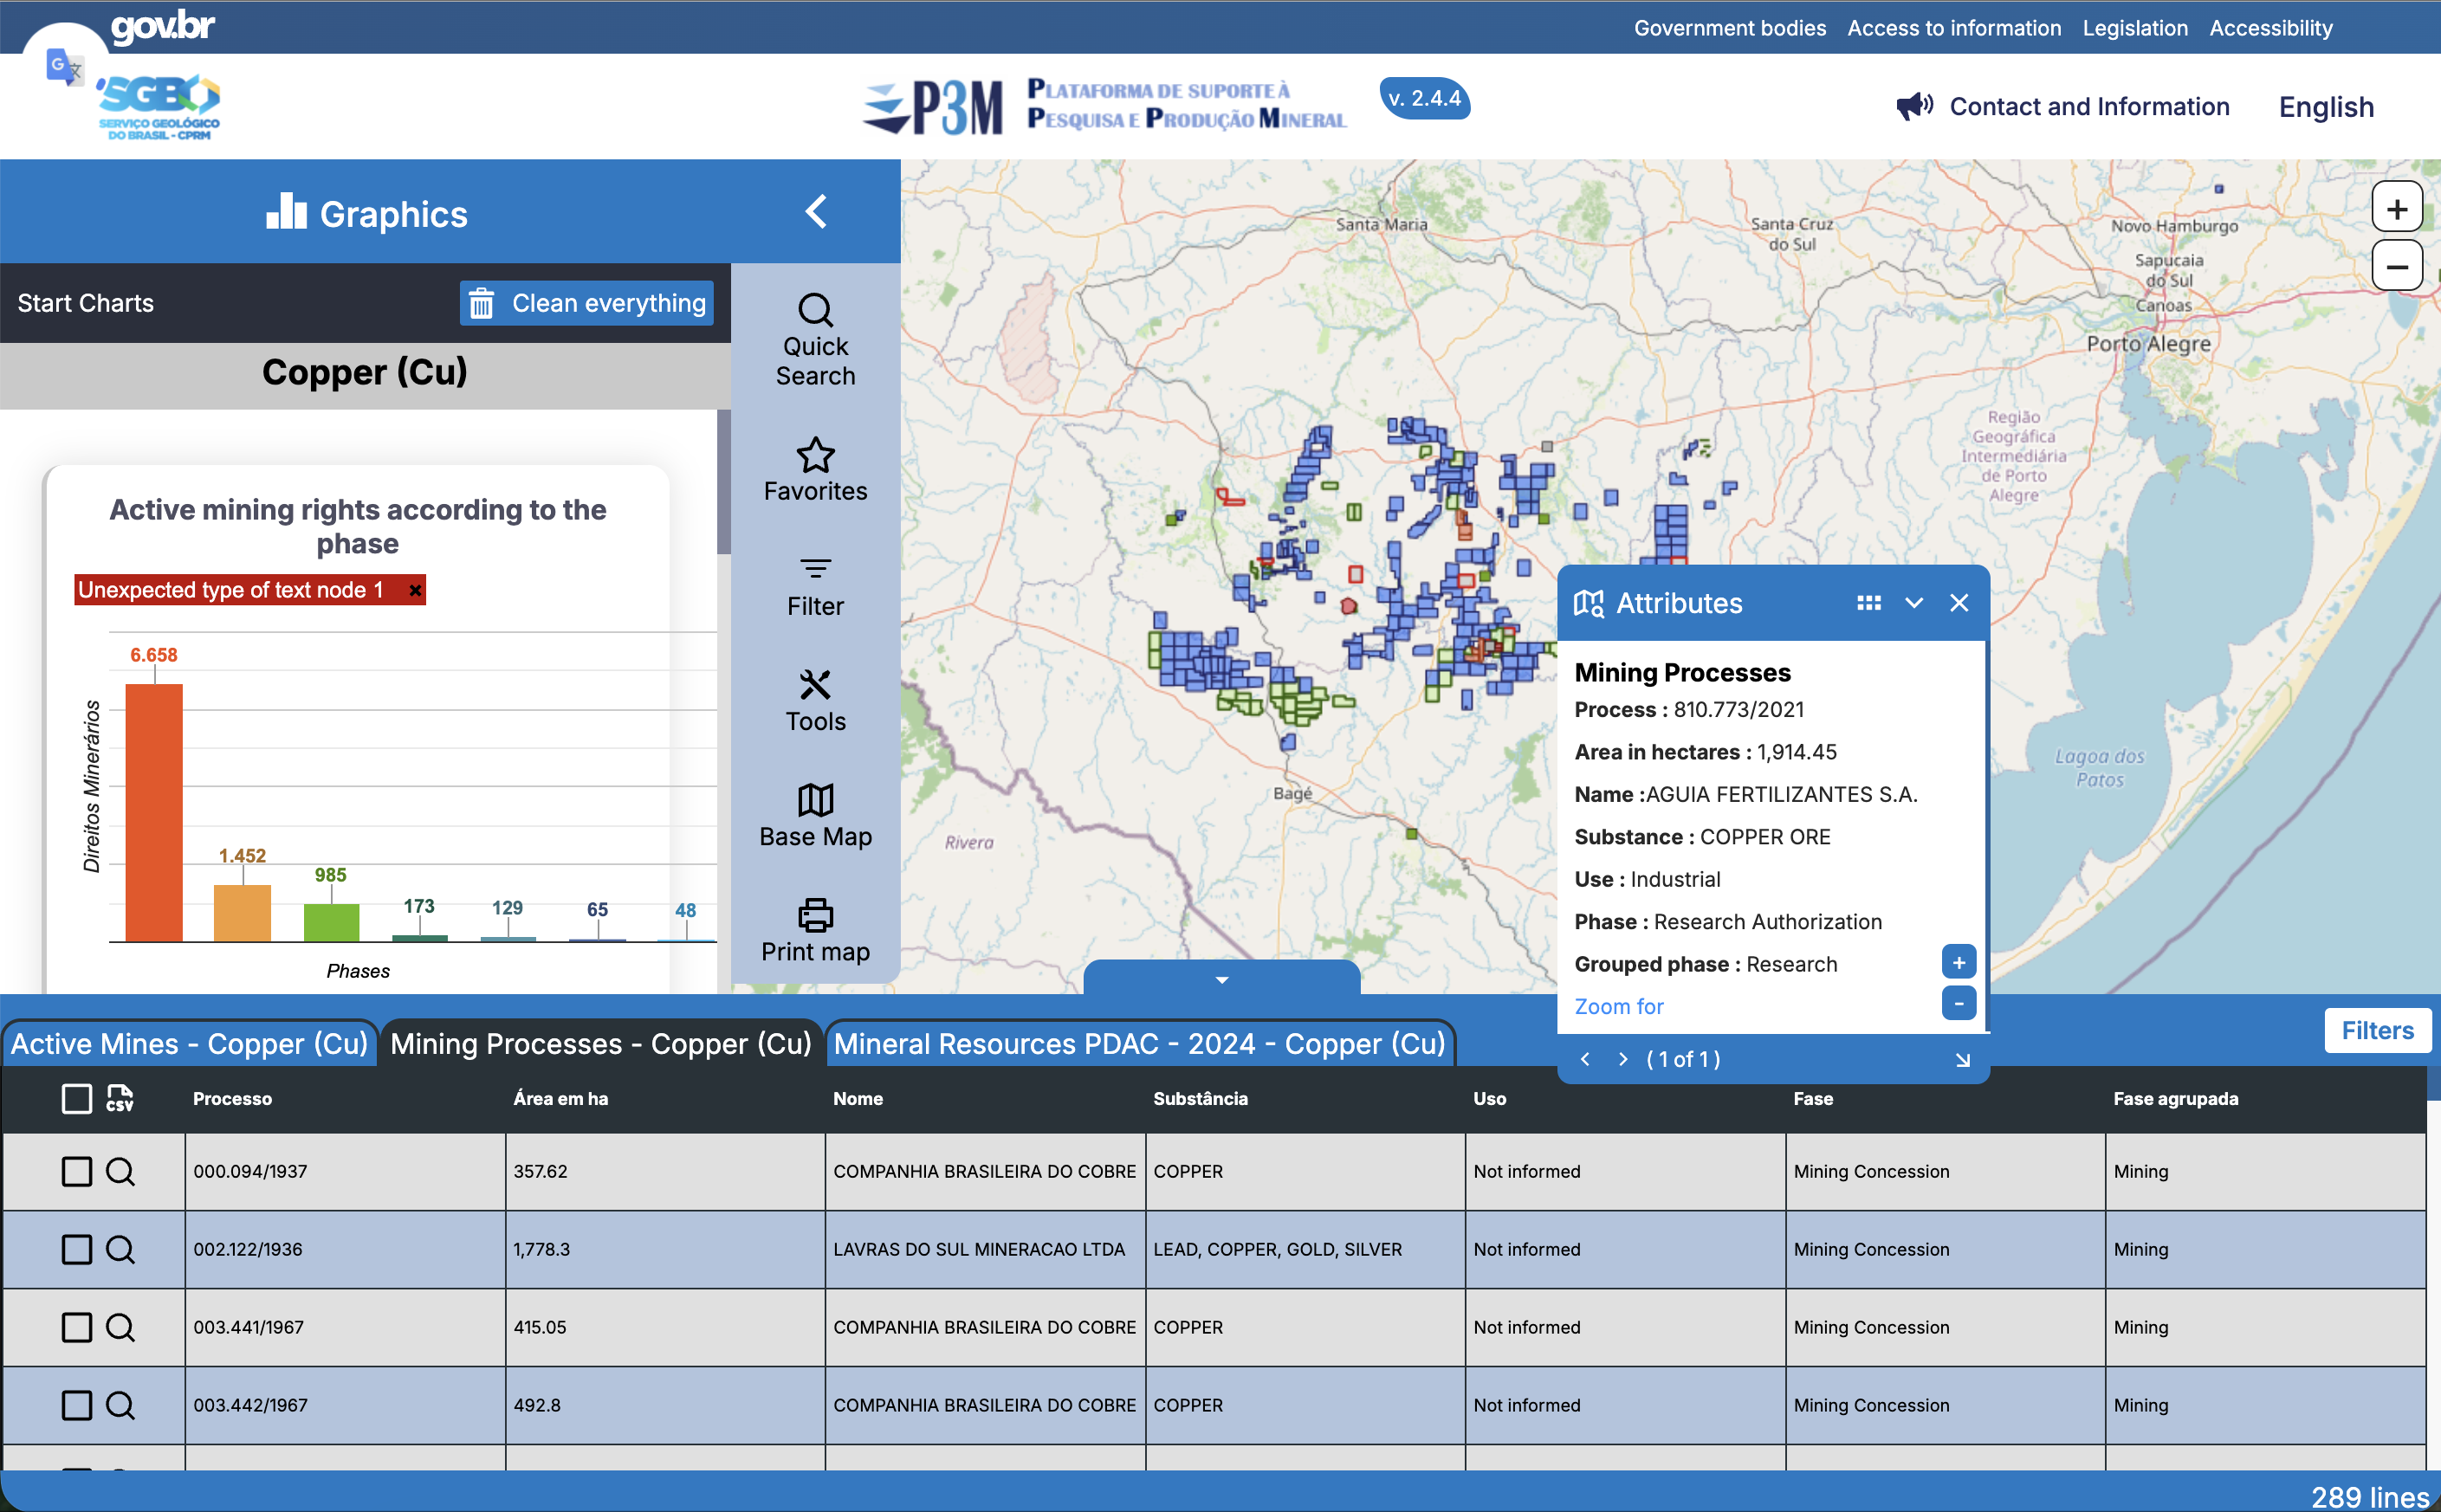
\includegraphics[width=1.0\columnwidth]{images/cobre-rs.png}
        \caption{Copper ventures on southern Brazil, according to P3M. On left panel, some relevant indicators for mineral industry, specified for the selected commodity}
        \label{fig:case-study-copper-rs}
    \end{center}
\end{figure}

Após a seleção......

In the specific case of Rio Grande do Sul, this information allowed for the identification of areas with a higher density of occurrences and geological indicators favorable to the presence of copper. Based on the preliminary geological analysis, it is possible to delineate regions of interest for research, evaluating their overlap with active mining rights and checking their legal availability.

The platform also allows for the activation of layers of legal and socio-environmental restrictions, such as indigenous lands, conservation units, settlement areas, and critical infrastructure, helping to exclude areas that are not suitable for applications (Figure~\ref{fig:case-study-copper-rs-support-layers}).

\begin{figure}[ht!]
    \begin{center}
        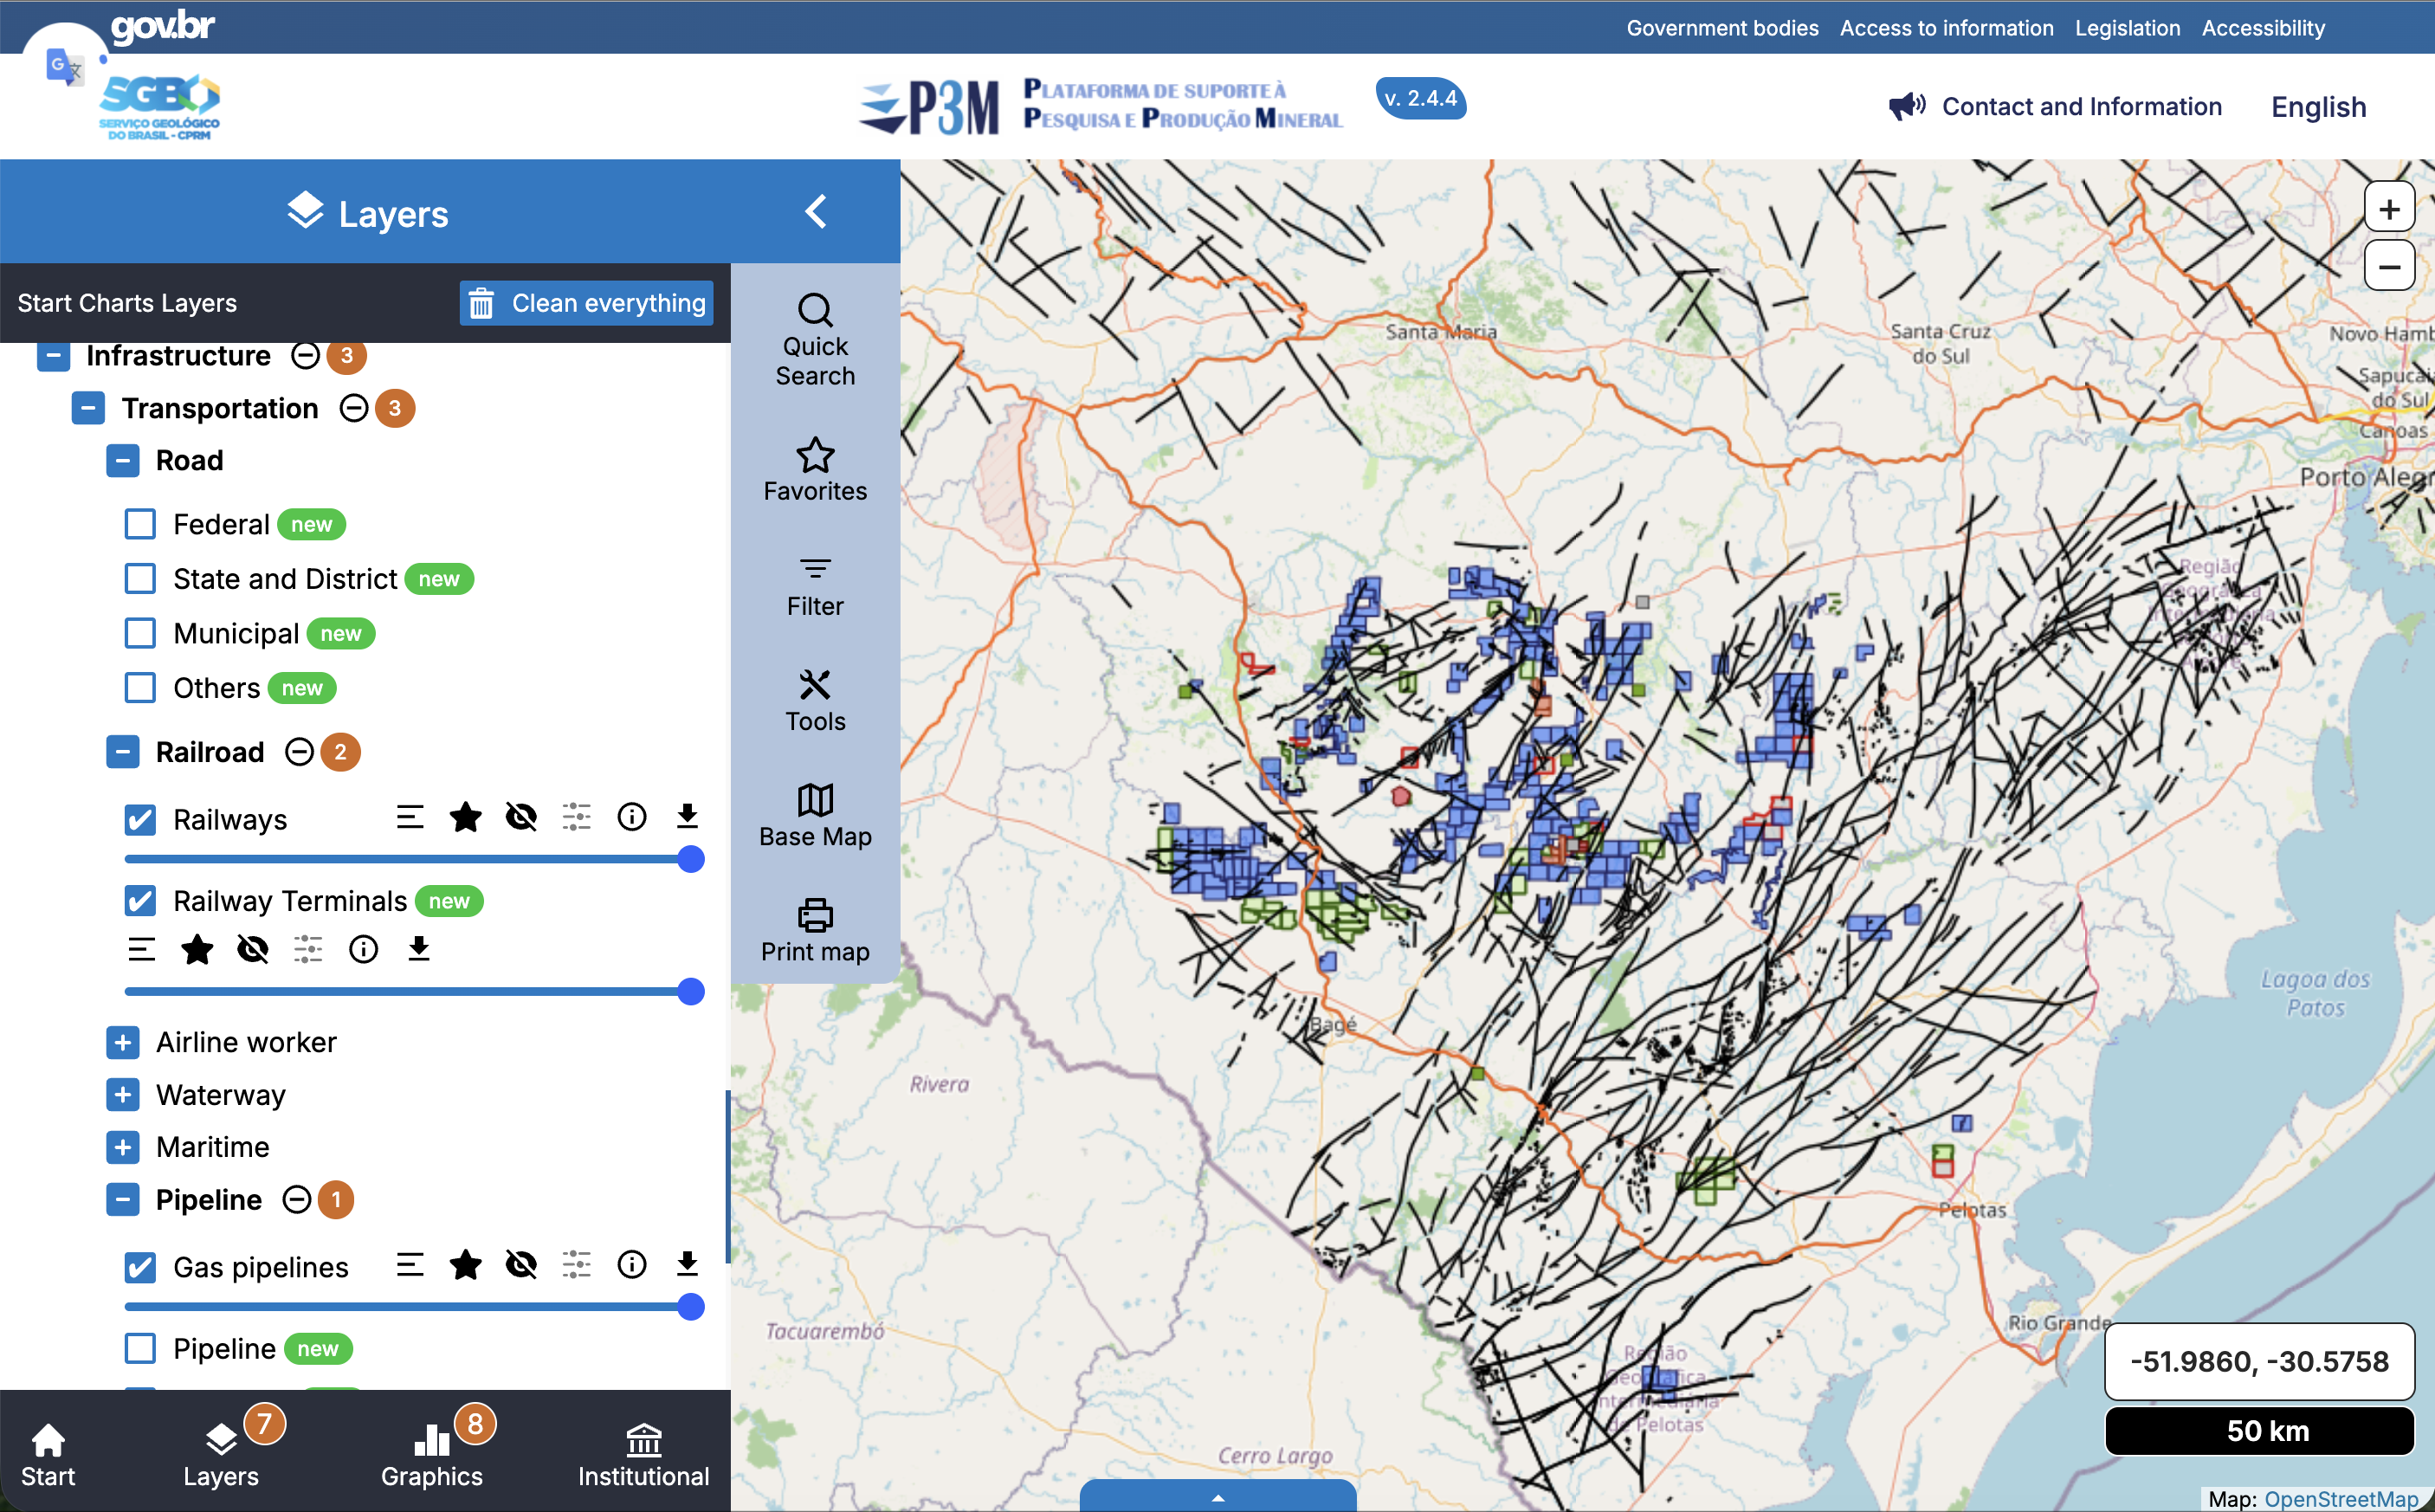
\includegraphics[width=1.0\columnwidth]{images/cobre-rs-camadas-apoio.png}
        \caption{Support layers, consumed from SGB's SDI (GeoNode), associated with mining layers.}
        \label{fig:case-study-copper-rs-support-layers}
    \end{center}
\end{figure}

Beyond the geological and legal aspects, the platform allows the user to examine logistical and market elements, such as transport infrastructure, ports, electricity grid, and the presence of consumer industries, providing input for a preliminary assessment of economic viability.

P3M's integrated statistics functionality also provides data on the evolution of copper requirements, the geoeconomic potential index of the substance, and the distribution of mining titles by process phase (Figures~\ref{fig:case-study-copper-rs-dashboard1} and~\ref{fig:case-study-copper-rs-dashboard2}).

\begin{figure}[ht!]
    \begin{center}
        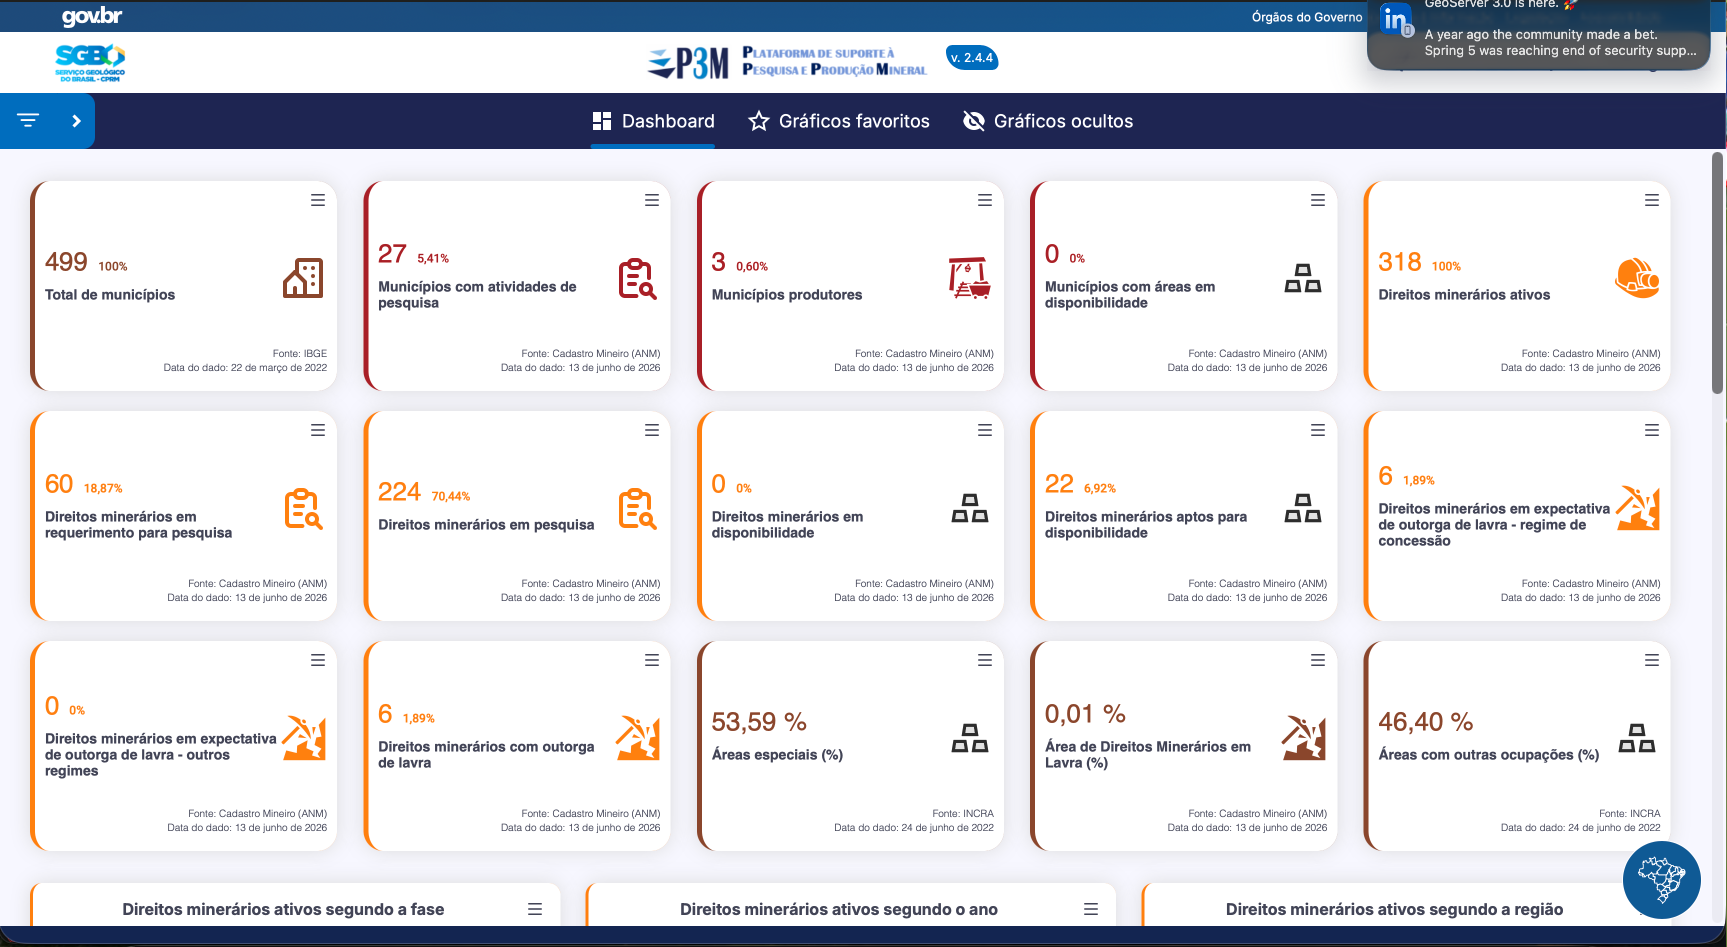
\includegraphics[width=1.0\columnwidth]{images/cobre-rs-dashboard1.png}
        \caption{Card section, with insights for mineral industry on P3M's dashboards.}
        \label{fig:case-study-copper-rs-dashboard1}
    \end{center}
\end{figure}

\begin{figure}[ht!]
    \begin{center}
        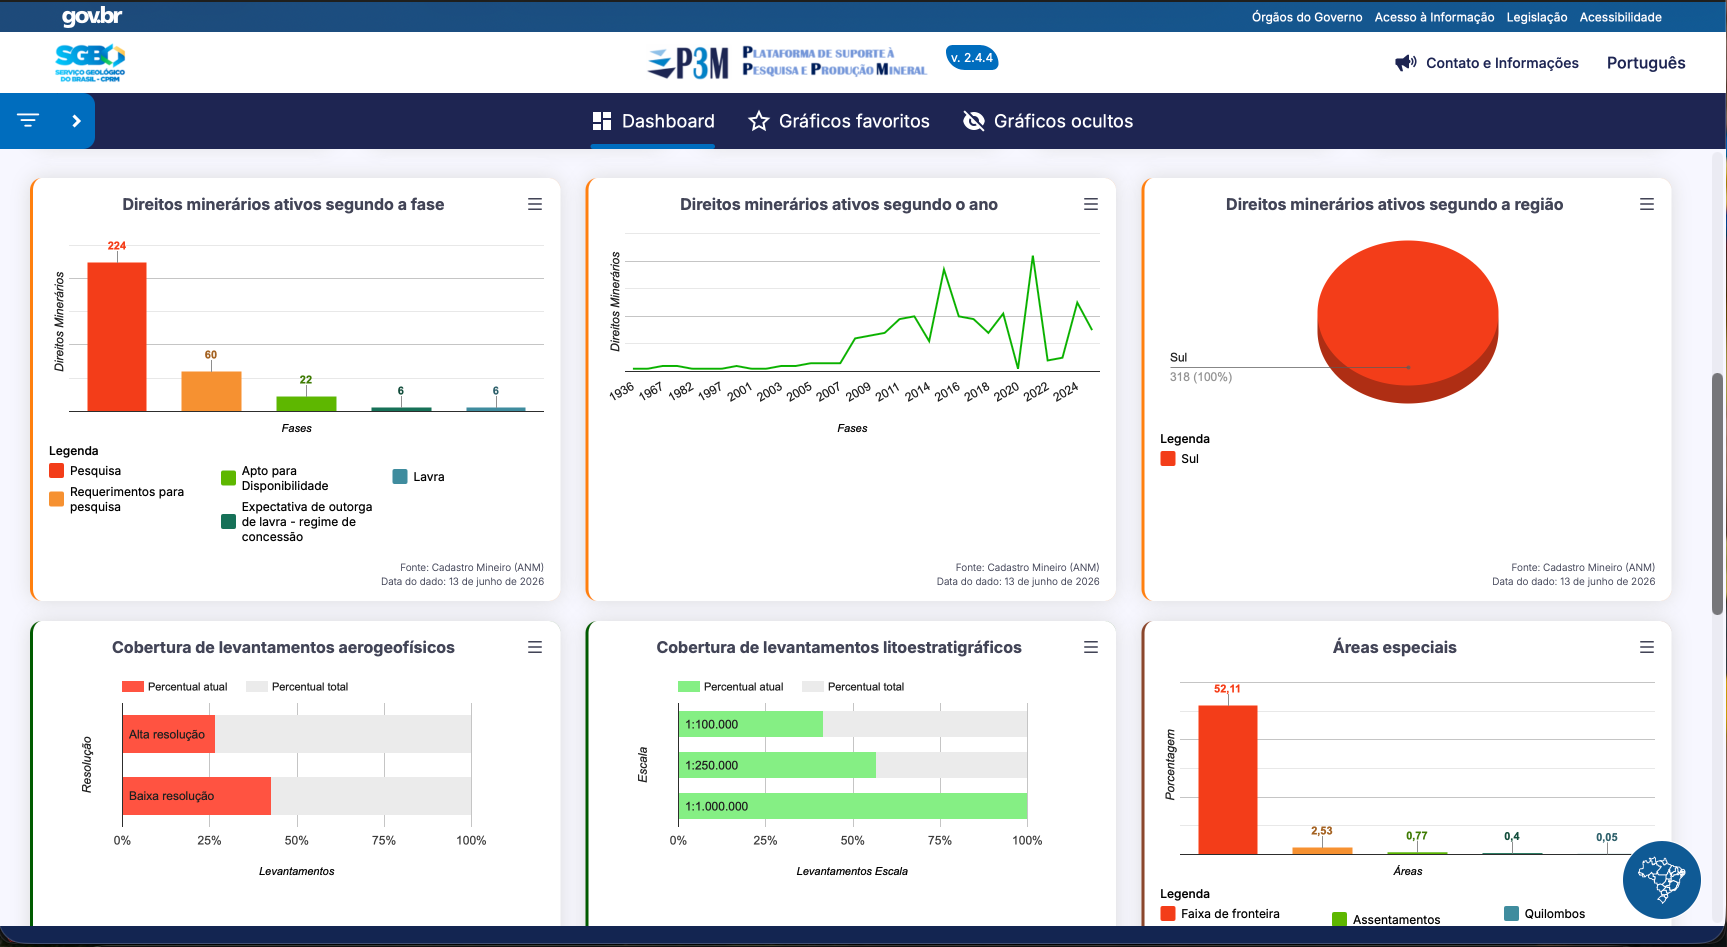
\includegraphics[width=1.0\columnwidth]{images/cobre-rs-dashboard2.png}
        \caption{Chart section, with insights for mineral industry on P3M's dashboards.}
        \label{fig:case-study-copper-rs-dashboard2}
    \end{center}
\end{figure}


\section{Conclusion}\label{CONCLUSION}

Finally, the P3M Platform, since its conception, has always been guided by the use of free and open-source libraries and frameworks to ensure transparency and interoperability. Alongside major FOSS4G projects, P3M stands out among the select group of data and service providers applied to Geology and Mining sectors by adopting frameworks that are free from restrictive licensing and bundled sales practices.

This study demonstrates that P3M is a robust tool for providing technical support to mineral research, especially in its initial phase, helping to select areas carefully and contributing to more efficient and informed decisions by investors and researchers \cite{carli2024}.

% References
{
	\begin{spacing}{1.17}
		\normalsize
		\bibliography{ISPRS_FOSS4G2026_mota_et_al_2026} % Include your own bibliography (*.bib), style is given in isprs.cls
	\end{spacing}
}
\end{document}
